\documentclass[11pt,a4paper]{article}

\usepackage[utf8]{inputenc}
\usepackage[T1]{fontenc}
\usepackage{lmodern}
\usepackage{amsmath,amssymb}
\usepackage{graphicx}
\usepackage{booktabs}
\usepackage{tabularx}
\usepackage{multirow}
\usepackage{float}
\usepackage[margin=1in]{geometry}

\graphicspath{{../}{../figures/}}

\renewcommand{\thetable}{S\arabic{table}}
\renewcommand{\thefigure}{S\arabic{figure}}

\title{Supplementary Materials\\HypEReg-TransMorph: A Hyperelastic-Regularized Transformer Framework for Folding-Suppressed Deformable Brain MRI Registration}
\author{}
\date{}

\begin{document}
\maketitle

\noindent This document accompanies the manuscript \emph{HypEReg-TransMorph: A Hyperelastic-Regularized Transformer Framework for Folding-Suppressed Deformable Brain MRI Registration}. Extended quantitative results, inferential tables (S1--S2), grouped-VOI mapping (S3), Figure~S1, OASIS protocol notes with Table~S5, bootstrap confidence intervals (Table~S6), Jacobian-ROI analysis placeholders (Table~S7), LPBA40 zero-shot placeholders (Table~S8), and implementation/profiling details are provided here as separate Supplementary Materials (they are not duplicated in the main journal PDF).

\section{Supplementary Experimental Details}
\subsection{Model and Environment Configuration}
To address reproducibility at full detail, we report \emph{all} explicit training-time and implementation hyperparameters used by the IXI HypEReg-TransMorph run (\texttt{IXI/TransMorph/train\_TransMorph\_her.py} with \texttt{CONFIGS\_TM['TransMorph']}).

\paragraph{Software and hardware environment.}
\begin{itemize}
\item Python 3.12.10.
\item PyTorch 2.12.0.dev20260408+cu128.
\item antspyx 0.6.3; SimpleITK 2.5.3.
\item Single GPU: NVIDIA RTX PRO 6000 Blackwell Workstation Edition (97,887 MiB VRAM), driver 591.86.
\end{itemize}

\paragraph{Data source, atlas resolution, and loaders.}
\begin{itemize}
\item IXI root directory resolved as \texttt{repo\_root/IXI\_data}; atlas resolved from \texttt{atlas.pkl} (fallback \texttt{altas.pkl}).
\item Training samples loaded from \texttt{IXI\_data/Train/*.pkl}; validation samples from \texttt{IXI\_data/Val/*.pkl}.
\item Batch size: 2 (training), 1 (validation).
\item DataLoader (train): \texttt{shuffle=True}, \texttt{num\_workers=4}, \texttt{pin\_memory=True}, \texttt{drop\_last=False} (default).
\item DataLoader (val): \texttt{shuffle=False}, \texttt{num\_workers=4}, \texttt{pin\_memory=True}, \texttt{drop\_last=True}.
\item Training transform pipeline: \texttt{RandomFlip(0)} then \texttt{NumpyType((np.float32, np.float32))}.
\item Validation transform pipeline: \texttt{Seg\_norm()} then \texttt{NumpyType((np.float32, np.int16))}.
\item \texttt{RandomFlip} implementation detail: independent Bernoulli flips for axes \((1,2,3)\) with \(\Pr(\text{flip along each axis})=0.5\).
\item \texttt{Seg\_norm} relabel table (in-order): \([0,2,3,4,5,7,8,10,11,12,13,14,15,16,17,18,24,26,28,30,31,41,42,43,44,46,47,49,50,51,52,53,54,58,60,62,63,72,77,80,85,251,252,253,254,255]\).
\end{itemize}

\paragraph{Optimization, schedule, and training loop controls.}
\begin{itemize}
\item Optimizer: Adam with AMSGrad (\texttt{optim.Adam(..., amsgrad=True)}).
\item Adam hyperparameters explicitly set: learning rate \(=1\times10^{-4}\), weight decay \(=0\).
\item Adam hyperparameters inherited from PyTorch defaults (not overridden): \(\beta_1=0.9\), \(\beta_2=0.999\), \(\epsilon=10^{-8}\).
\item Epoch controls: \texttt{epoch\_start=0}, \texttt{max\_epoch=500}, \texttt{cont\_training=False}.
\item LR schedule (applied every training iteration): polynomial decay
\[
\mathrm{lr}(e)=\mathrm{INIT\_LR}\cdot\left(1-\frac{e}{\mathrm{MAX\_EPOCHES}}\right)^{0.9},
\]
with \texttt{round(..., 8)} applied in code.
\item Bidirectional optimization per mini-batch: one step for \(x\rightarrow y\), one step for \(y\rightarrow x\), each with independent \texttt{zero\_grad()}, \texttt{backward()}, \texttt{step()}.
\item Random global seed: the released training script follows the upstream TransMorph reference implementation and does not pin a single global PyTorch/NumPy/Python seed; reproducibility is supported at the level of the released checkpoint, the deterministic evaluation pipeline, and per-case metric exports. A multi-seed extension (\(\geq 3\) re-trainings) is identified in the main-paper limitations as a complementary direction.
\end{itemize}

\paragraph{Loss composition (all coefficients and internal settings).}
Total objective per direction:
\[
\mathcal{L}_{\mathrm{total}}
=
1.0\cdot\mathcal{L}_{\mathrm{sim}}
+1.0\cdot\mathcal{L}_{\mathrm{grad}}
+1.0\cdot\mathcal{L}_{\mathrm{HypEReg}}.
\]
\begin{itemize}
\item Similarity term: \texttt{losses.NCC\_vxm(win=None)}.
\item NCC window: \([9,9,9]\) (auto-selected from \texttt{win=None} for 3D).
\item NCC return form: negative mean squared local cross-correlation (\(-\overline{\mathrm{LCC}^2}\)); denominator stabilizer \(=10^{-5}\).
\item Smoothness term: \texttt{losses.Grad3d(penalty='l2', loss\_mult=None)}.
\item Grad3d form: mean squared first-order finite differences along x/y/z, then divided by 3.
\item Hyperelastic term class: \texttt{HyperelasticLoss(alpha\_length=0.0, beta\_volume=0.02, gamma\_fold=20.0)} (the \texttt{alpha\_length} argument is the code-level knob for the BMR length surrogate; it is fixed to 0.0, equivalent to excluding the length term from the HypEReg construction as described in \S2.4 of the main text).
\item Hyperelastic internal defaults (not overridden): \texttt{eps=1e-3}, \texttt{fold\_power=2}, \texttt{penalty\_type='rational'}.
\item Active HypEReg weights in this operating point: \(\beta=0.02\), \(\gamma=20\), \(\epsilon=10^{-3}\).
\item Jacobian computation in HER: forward finite differences on interior lattice \((D-1,H-1,W-1)\), with \(J=\det(I+\nabla u)\).
\item Volume penalty: \((J-1)^2/\max(J,\epsilon)\) with \(\epsilon=10^{-3}\).
\item Folding penalty: \(\mathrm{ReLU}(\epsilon-J)^2\) with \(\epsilon=10^{-3}\).
\end{itemize}

\paragraph{Model architecture hyperparameters (TransMorph backbone).}
The run uses \texttt{config = CONFIGS\_TM['TransMorph']} from \texttt{configs\_TransMorph.py}, i.e.:
\begin{itemize}
\item \texttt{if\_transskip=True}, \texttt{if\_convskip=True}.
\item \texttt{patch\_size=4}, \texttt{in\_chans=2}, \texttt{img\_size=(160,192,224)}.
\item \texttt{embed\_dim=96}, \texttt{depths=(2,2,4,2)}, \texttt{num\_heads=(4,4,8,8)}.
\item \texttt{window\_size=(5,6,7,7)} (as defined in the released config).
\item \texttt{mlp\_ratio=4}, \texttt{pat\_merg\_rf=4}, \texttt{reg\_head\_chan=16}.
\item \texttt{qkv\_bias=False}, \texttt{drop\_rate=0}, \texttt{drop\_path\_rate=0.3}.
\item Positional/normalization/checkpoint flags: \texttt{ape=False}, \texttt{spe=False}, \texttt{rpe=True}, \texttt{patch\_norm=True}, \texttt{use\_checkpoint=False}.
\item Feature output stages: \texttt{out\_indices=(0,1,2,3)}.
\item Trainable parameter count noted in the config comment: 15,201,579.
\end{itemize}

\paragraph{Warping kernels, logging, and checkpoint policy.}
\begin{itemize}
\item Two registration utility kernels instantiated during training: nearest-neighbor warp (labels) and bilinear warp (grid/intensity visualization).
\item TensorBoard logging path: \texttt{logs/TransMorph\_IXI\_HER\_ncc\_1.0\_grad\_1.0\_her\_1.0\_a0\_b0.02\_g20/}.
\item Checkpoint path: \texttt{experiments/TransMorph\_IXI\_HER\_ncc\_1.0\_grad\_1.0\_her\_1.0\_a0\_b0.02\_g20/}.
\item Model-selection metric: best validation Dice (\texttt{best\_dsc}).
\item Checkpoint filename template: \texttt{dsc\{:.3f\}.pth.tar}; retention cap \texttt{max\_model\_num=8} with oldest-file deletion.
\end{itemize}

\paragraph{Inference/profiling controls (for reported runtime numbers).}
\begin{itemize}
\item Inference benchmarks use the standardized evaluation script in the repository with harmonized metric definitions across models.
\item Isolated forward profiling is performed with \texttt{torch.no\_grad()} enabled, label-warp/metric kernels excluded, and \texttt{torch.cuda.max\_memory\_allocated()} reset before each warm-started measurement.
\item Pure-forward runtime / peak GPU memory on the reported NVIDIA RTX PRO 6000 Blackwell hardware: HypEReg-TransMorph \(0.0822\) s / \(5.685\) GB; TransMorph \(0.0822\) s / \(5.685\) GB; TransMorphBayes \(0.0852\) s / \(6.042\) GB. Values are averages of \(20\) repeated calls on synthetic inputs of size \(1\times2\times160\times192\times224\) following 5 warm-up iterations. The two TransMorph variants share the same forward graph and therefore yield identical timings (parameter count is \(46.771\)\,M and \(46.773\)\,M, respectively).
\end{itemize}

\begin{table}[H]
\caption{Baseline checkpoint provenance (IXI). Checkpoint paths are resolved by the evaluation adapters under \texttt{IXI/adapters/}.\label{tab:s2b_provenance}}
\scriptsize
\setlength{\tabcolsep}{4pt}
\renewcommand{\arraystretch}{1.1}
\begin{tabularx}{\textwidth}{lXX}
\toprule
\textbf{Model} & \textbf{Adapter module} & \textbf{Checkpoint path / source} \\
\midrule
HypEReg-TransMorph & \texttt{IXI/adapters/transmorph\_her.py} & \texttt{IXI/TransMorph/experiments/TransMorph\_IXI\_HER\_ncc\_1.0\_grad\_1.0\_her\_1.0\_a0\_b0.02\_g20/dsc0.743.pth.tar} \\
TransMorph & \texttt{IXI/adapters/transmorph\_original.py} & Prefer uploaded \texttt{IXI/TransMorph/experiments/TransMorph\_Validation\_dsc0.744.pth.tar}; fallback to latest under \texttt{IXI/TransMorph/experiments/TransMorph\_IXI\_ncc\_1.0\_grad\_1.0/} \\
TransMorphBayes & \texttt{IXI/adapters/transmorphbayes.py} & Prefer uploaded \texttt{IXI/TransMorph/experiments/TransMorph\_Bayes\_Validation\_dsc0.743.pth.tar}; fallback to latest under \texttt{IXI/TransMorph/experiments/TransMorphBayes\_ncc\_1\_diffusion\_1/} \\
MIDIR & \texttt{IXI/adapters/midir.py} & \texttt{IXI/Baseline\_registration\_methods/MIDIR/MIDIR\_Validation\_dsc0.733.pth.tar} \\
CycleMorph & \texttt{IXI/adapters/cyclemorph.py} & \texttt{IXI/Baseline\_registration\_methods/CycleMorph/CycleMorph\_Validation\_dsc0.729.pth.tar} \\
VoxelMorph-1 & \texttt{IXI/adapters/voxelmorph\_1.py} & \texttt{IXI/Baseline\_registration\_methods/VoxelMorph/VoxelMorph\_1\_Validation\_dsc0.720.pth.tar} \\
CoTr & \texttt{IXI/adapters/cotr.py} & \texttt{IXI/Baseline\_Transformers/models/CoTr/CoTr\_Validation\_dsc0.730.pth.tar} \\
nnFormer & \texttt{IXI/adapters/nnformer.py} & \texttt{IXI/Baseline\_Transformers/models/nnFormer/nnFormer\_Validation\_dsc0.739.pth.tar} \\
PVT & \texttt{IXI/adapters/pvt.py} & \texttt{IXI/Baseline\_Transformers/PVT\_Validation\_dsc0.720.pth.tar} \\
SyN (ANTs) & \texttt{IXI/adapters/syn\_legacy\_to\_per\_case.py} & Legacy outputs converted from \texttt{IXI/Eval\_Results/comprehensive\_syn\_lddmm/SyN\_IXI/} (no learned checkpoint) \\
\bottomrule
\end{tabularx}
\end{table}

\section{Figure S1: Descriptive IXI Overview}

\begin{figure}[H]
\centering
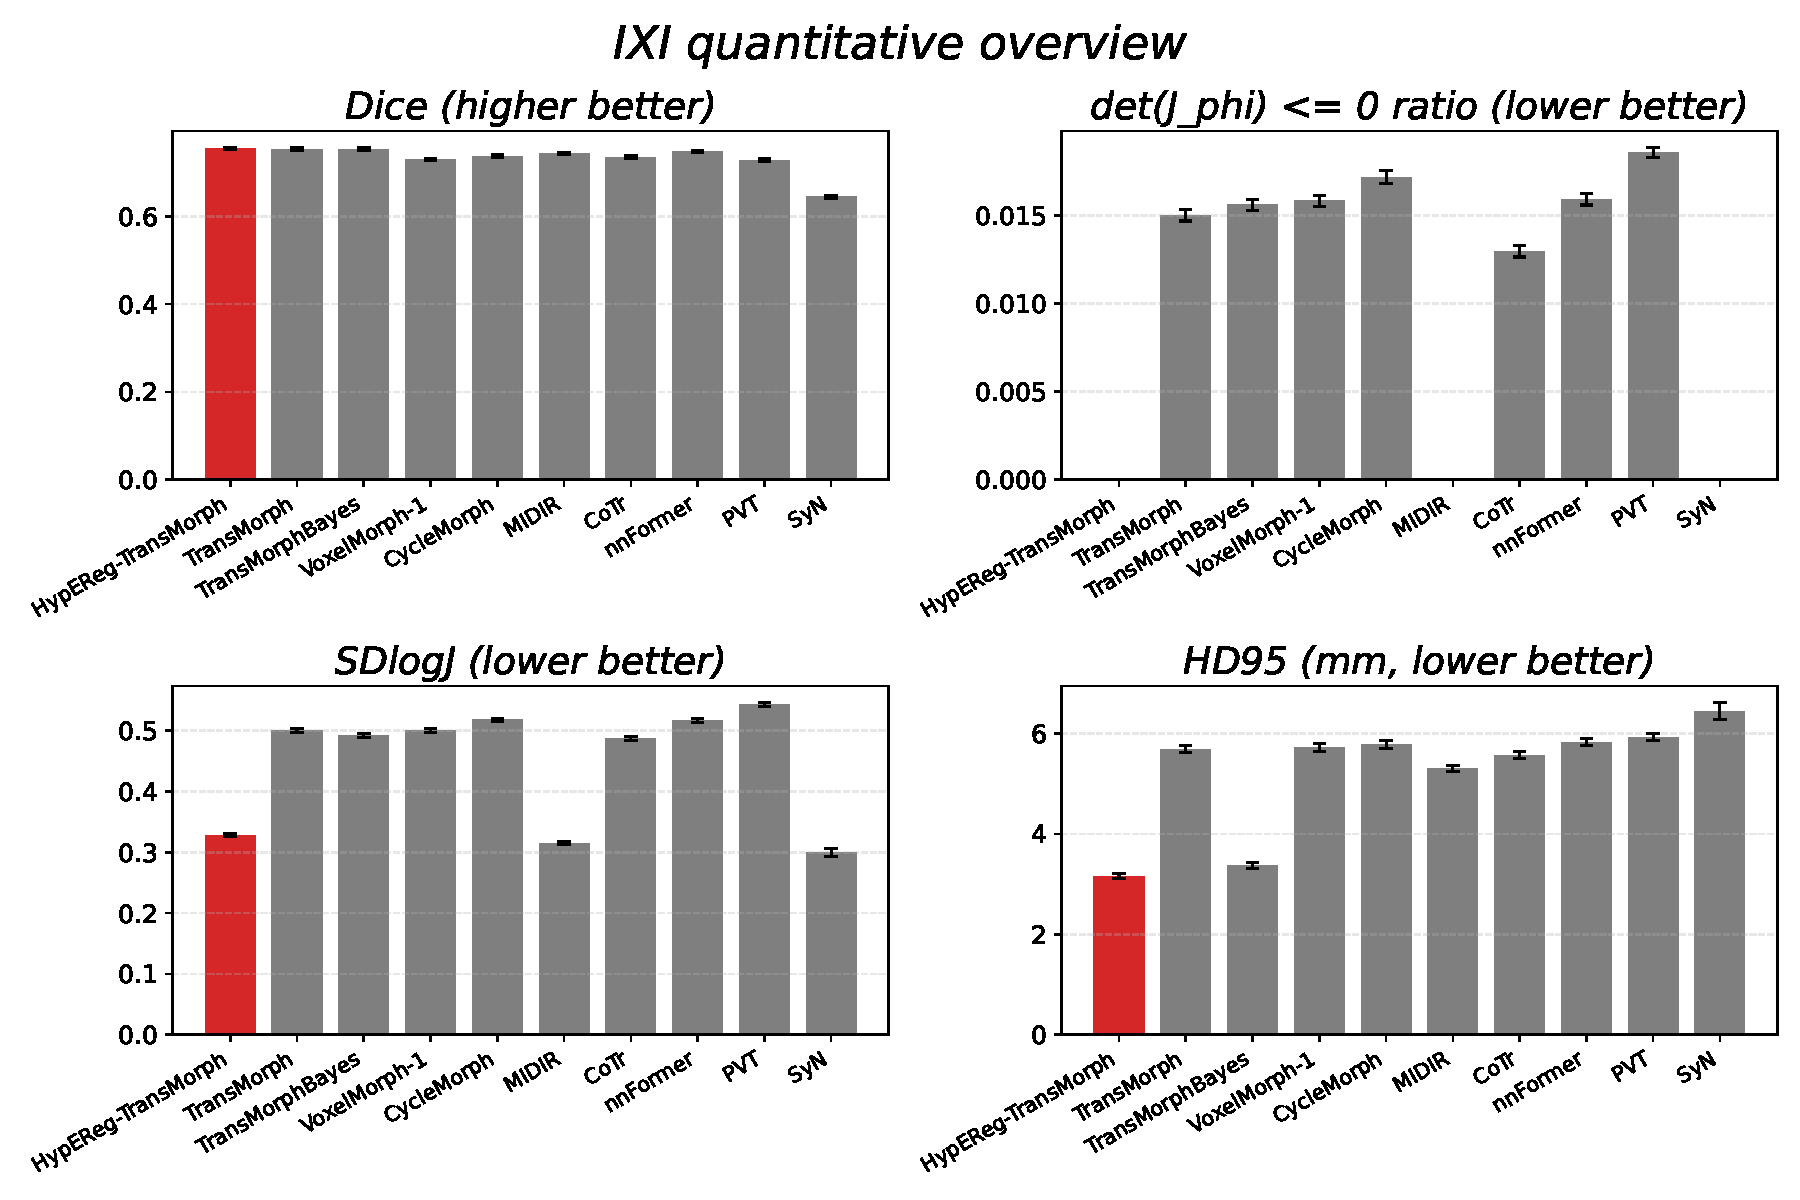
\includegraphics[width=0.99\textwidth]{figures/fig5_metrics.pdf}
\caption{Descriptive IXI quantitative overview (Dice, non-positive Jacobian determinant ratio, SDlogJ, and HD95). Bars include standard-error error bars for visual uncertainty context. (HER-TransMorph in the panel labels denotes HypEReg-TransMorph.)}
\end{figure}

\section{Inferential Statistics (HypEReg-TransMorph vs.\ Baselines)}

\noindent\textbf{Metric definitions (to avoid naming ambiguity).} In this Supplementary section, \texttt{dice\_mean} denotes the per-subject mean Dice computed over the full 46-label FreeSurfer-compatible label set (columns \texttt{dice\_0}--\texttt{dice\_45} in \texttt{per\_case.csv}), whereas the main paper reports \emph{grouped Dice} averaged over 17 grouped VOIs (Table~\ref{tab2} in the main text). The two numbers therefore have different scales and are not directly comparable.

\begin{table}[H]
\caption{Auxiliary deformation and surface metrics on IXI (mean\(\pm\)std over subjects). This table reports NSD@1\,mm and additional deformation-regularity descriptors that are referenced in the main text but not included in Table~2.\label{tab:s0_aux_metrics}}
\scriptsize
\setlength{\tabcolsep}{3pt}
\renewcommand{\arraystretch}{1.1}
\begin{tabularx}{\textwidth}{lXXXXXXXX}
\toprule
\textbf{Model} & \textbf{NSD@1\,mm\(\uparrow\)} & \textbf{Bending\(\downarrow\)} & \textbf{MADiv\(\downarrow\)} & \(\boldsymbol{J_{\min}}\) & \(\boldsymbol{J_{p01}}\) & \(\boldsymbol{J_{p99}}\) & \(\boldsymbol{J_{\max}}\)\\
\midrule
HypEReg-TransMorph (HER\_dsc0743) & 0.8480 \(\pm\) 0.0317 & 0.0031 \(\pm\) 0.0001 & 0.1772 \(\pm\) 0.0114 & -0.2700 \(\pm\) 0.1496 & 0.2754 \(\pm\) 0.0268 & 2.1284 \(\pm\) 0.0669 & 18.6155 \(\pm\) 2.9607\\
TransMorphBayes & 0.8462 \(\pm\) 0.0347 & 0.0050 \(\pm\) 0.0003 & 0.2341 \(\pm\) 0.0114 & -6.6766 \(\pm\) 2.2896 & -0.0871 \(\pm\) 0.0555 & 2.5926 \(\pm\) 0.0764 & 46.0976 \(\pm\) 9.2892\\
HER\_active & 0.7715 \(\pm\) 0.0398 & 0.0036 \(\pm\) 0.0001 & 0.1719 \(\pm\) 0.0077 & -0.1754 \(\pm\) 0.0993 & 0.3433 \(\pm\) 0.0196 & 2.1054 \(\pm\) 0.0979 & 12.3397 \(\pm\) 2.2249\\
HERGRAD\_active & 0.7612 \(\pm\) 0.0403 & 0.0019 \(\pm\) 0.0001 & 0.1549 \(\pm\) 0.0065 & -0.1014 \(\pm\) 0.0928 & 0.3729 \(\pm\) 0.0187 & 2.0257 \(\pm\) 0.0840 & 8.4640 \(\pm\) 1.1222\\
HERGRAD\_foldonly & 0.7242 \(\pm\) 0.0424 & 0.0041 \(\pm\) 0.0001 & 0.2367 \(\pm\) 0.0064 & -1.2721 \(\pm\) 0.3317 & 0.0776 \(\pm\) 0.0232 & 2.5189 \(\pm\) 0.0782 & 19.8379 \(\pm\) 2.8103\\
\bottomrule
\end{tabularx}
\parbox{\textwidth}{\footnotesize Bending = voxel-averaged bending energy; MADiv = mean absolute divergence of the displacement field; NSD@1\,mm computed with \(\tau=1\) mm. Values are taken from the consolidated comprehensive-evaluation tables generated by \texttt{IXI/analysis\_comprehensive}.}
\end{table}

\begin{table}[H]
\caption{Inferential summary for TransMorphBayes and MIDIR (mean\(\pm\)std, aligned median difference, Wilcoxon \(p\), Benjamini--Hochberg \(q\), and matched-pairs rank-biserial effect). HypEReg-TransMorph denotes the proposed model.}
\scriptsize
\setlength{\tabcolsep}{3pt}
\renewcommand{\arraystretch}{1.1}
\begin{tabularx}{\textwidth}{llXXXX}
\toprule
\textbf{Metric} & \textbf{Baseline} & \textbf{HypEReg mean\(\pm\)std} & \textbf{Baseline mean\(\pm\)std} & \textbf{Median diff (aligned)} & \textbf{\(p\)/\(q\)/effect}\\
\midrule
dice\_mean & TransMorphBayes (uploaded ckpt) & 0.5765\(\pm\)0.0301 & 0.5731\(\pm\)0.0313 & 0.00280 & \(6.58\times10^{-10}\) / \(6.58\times10^{-10}\) / 0.6636\\
non\_jec & TransMorphBayes (uploaded ckpt) & \(1.46\times10^{-5}\)\(\pm\)\(7.37\times10^{-6}\) & 0.01510\(\pm\)0.00329 & 0.01489 & \(1.31\times10^{-20}\) / \(3.28\times10^{-20}\) / 1.0000\\
SDlogJ & TransMorphBayes (uploaded ckpt) & 0.3280\(\pm\)0.0221 & 0.4934\(\pm\)0.0334 & 0.16325 & \(1.31\times10^{-20}\) / \(3.28\times10^{-20}\) / 1.0000\\
HD95\_mean & TransMorphBayes (uploaded ckpt) & 5.3234\(\pm\)0.6936 & 5.7246\(\pm\)0.7604 & 0.33877 & \(1.77\times10^{-18}\) / \(2.94\times10^{-18}\) / 0.9424\\
ASSD\_mean & TransMorphBayes (uploaded ckpt) & 1.3570\(\pm\)0.1770 & 1.4160\(\pm\)0.1832 & 0.06143 & \(2.98\times10^{-11}\) / \(3.72\times10^{-11}\) / 0.7142\\
\midrule
dice\_mean & MIDIR & 0.5765\(\pm\)0.0301 & 0.5643\(\pm\)0.0244 & 0.01166 & \(3.79\times10^{-18}\) / \(7.76\times10^{-18}\) / 0.9331\\
non\_jec & MIDIR & \(1.46\times10^{-5}\)\(\pm\)\(7.37\times10^{-6}\) & 0.0000\(\pm\)0.0000 & \(-1.31\times10^{-5}\) & \(1.31\times10^{-20}\) / \(3.69\times10^{-20}\) / -1.0000\\
SDlogJ & MIDIR & 0.3280\(\pm\)0.0221 & 0.3148\(\pm\)0.0242 & -0.01365 & \(4.84\times10^{-20}\) / \(1.28\times10^{-19}\) / -0.9850\\
HD95\_mean & MIDIR & 5.3234\(\pm\)0.6936 & 5.3028\(\pm\)0.6139 & -0.00855 & 0.5767 / 0.5898 / -0.0600\\
ASSD\_mean & MIDIR & 1.3570\(\pm\)0.1770 & 1.4100\(\pm\)0.1585 & 0.06514 & \(3.58\times10^{-9}\) / \(4.36\times10^{-9}\) / 0.6342\\
\bottomrule
\end{tabularx}
\parbox{\textwidth}{\footnotesize Aligned median difference is oriented so positive values indicate HypEReg-TransMorph improvement for the given metric direction. The effect is matched-pairs rank-biserial correlation. Pair counts: \(n=115\) for both baselines in this table.}
\end{table}

\begin{table}[H]
\caption{Selected paired comparisons (Wilcoxon signed-rank with Benjamini--Hochberg FDR). Positive signed effect indicates HypEReg-TransMorph improvement under metric-aligned directionality; signed effect is matched-pairs rank-biserial correlation.}
\scriptsize
\setlength{\tabcolsep}{3pt}
\begin{tabularx}{\textwidth}{llcccc}
\toprule
\textbf{Metric} & \textbf{Baseline} & \textbf{Median paired diff (aligned)} & \textbf{p-value} & \textbf{q-value} & \textbf{Signed effect}\\
\midrule
non\_jec & TransMorph & 0.014747 & \(1.31\times 10^{-20}\) & \(3.69\times 10^{-20}\) & 1.0000 \\
SDlogJ & TransMorph & 0.170655 & \(1.31\times 10^{-20}\) & \(3.69\times 10^{-20}\) & 1.0000 \\
HD95\_mean & TransMorph & 0.319583 & \(3.77\times 10^{-17}\) & \(7.08\times 10^{-17}\) & 0.9046 \\
ASSD\_mean & TransMorph & 0.051747 & \(6.09\times 10^{-11}\) & \(7.83\times 10^{-11}\) & 0.7028 \\
\midrule
non\_jec & MIDIR & -0.000013 & \(1.31\times 10^{-20}\) & \(3.69\times 10^{-20}\) & -1.0000 \\
SDlogJ & MIDIR & -0.013652 & \(4.84\times 10^{-20}\) & \(1.28\times 10^{-19}\) & -0.9850 \\
HD95\_mean & MIDIR & -0.008554 & 0.5767 & 0.5898 & -0.0600 \\
ASSD\_mean & MIDIR & 0.065138 & \(3.58\times 10^{-9}\) & \(4.36\times 10^{-9}\) & 0.6342 \\
\midrule
non\_jec & TransMorph (uploaded ckpt) & 0.014747 & \(1.31\times 10^{-20}\) & \(2.63\times 10^{-20}\) & 1.0000 \\
dice\_mean & TransMorph (uploaded ckpt) & 0.002326 & \(6.88\times 10^{-7}\) & \(6.88\times 10^{-7}\) & 0.5334 \\
non\_jec & TransMorphBayes (uploaded ckpt) & 0.014714 & \(1.31\times 10^{-20}\) & \(2.63\times 10^{-20}\) & 1.0000 \\
dice\_mean & TransMorphBayes (uploaded ckpt) & 0.002706 & \(1.74\times 10^{-10}\) & \(2.32\times 10^{-10}\) & 0.6858 \\
\midrule
non\_jec & SyN & -0.000012 & \(8.00\times 10^{-16}\) & \(1.24\times 10^{-15}\) & -0.8654 \\
SDlogJ & SyN & -0.045599 & \(3.09\times 10^{-5}\) & \(3.31\times 10^{-5}\) & -0.4477 \\
HD95\_mean & SyN & 0.705730 & \(1.31\times 10^{-7}\) & \(1.47\times 10^{-7}\) & 0.5670 \\
ASSD\_mean & SyN & -0.111801 & 0.6572 & 0.6572 & 0.0477 \\
\bottomrule
\end{tabularx}
\end{table}

\noindent\footnotesize Full inferential outputs across all exported metric-baseline pairs are provided in the supplementary release package. Additional uploaded-checkpoint paired results for TransMorph and TransMorphBayes (Dice and non-positive Jacobian ratio) are included with corresponding subject-level inputs. Repeated values such as \(p=1.31\times 10^{-20}\) occur when the two-sided Wilcoxon test reaches the practical floating-point floor under near-complete sign consistency for \(n=115\), and should be interpreted as extremely small \(p\)-values.

\section{Table S3: Grouped-VOI Mapping}

\begin{table}[H]
\caption{Grouped-VOI mapping used for grouped Dice reporting.}
\scriptsize
\begin{tabularx}{\textwidth}{lX}
\toprule
\textbf{Grouped VOI} & \textbf{FreeSurfer-compatible label IDs} \\
\midrule
Brain-Stem & 16 \\
Thalamus & 10, 49 \\
Cerebellum-Cortex & 8, 47 \\
Cerebral-White-Matter & 2, 41 \\
Cerebellum-White-Matter & 7, 46 \\
Putamen & 12, 51 \\
VentralDC & 28, 60 \\
Pallidum & 13, 52 \\
Caudate & 11, 50 \\
Lateral-Ventricle & 4, 43 \\
Hippocampus & 17, 53 \\
3rd-Ventricle & 14 \\
4th-Ventricle & 15 \\
Amygdala & 18, 54 \\
Cerebral-Cortex & 3, 42 \\
CSF & 24 \\
choroid-plexus & 31, 63 \\
\bottomrule
\end{tabularx}
\end{table}

\section{OASIS Cross-Cohort Training and Environment}
The OASIS HypEReg-TransMorph run mirrors the IXI configuration in \texttt{OASIS/TransMorph/train\_TransMorph\_her.py} with \texttt{CONFIGS\_TM['TransMorph']}, the same Adam/AMSGrad settings, polynomial LR decay, bidirectional updates, and HypEReg weights $(\beta,\gamma,\epsilon)=(0.02,20,10^{-3})$. Software versions should match the IXI block where possible (Python~3.12.x, PyTorch with a CUDA build appropriate to the host GPU, antspyx for SyN, SimpleITK for affine). Checkpoints are written under \texttt{OASIS/TransMorph/experiments/}; evaluation is driven by \texttt{OASIS/export\_displacements.py}, \texttt{OASIS/eval\_oasis.py}, \texttt{OASIS/run\_full\_eval.ps1}, and \texttt{OASIS/oasis\_run\_stats.py}.

\section{Table S5: OASIS Paired Wilcoxon / BH-FDR}

\noindent Reference model: \texttt{transmorph\_her\_oasis} (HypEReg-TransMorph, OASIS-retrained). All pairs $n{=}19$. Only significant contrasts ($q_{\mathrm{BH}}<0.05$) shown; sign of direction: $+$ = HypEReg-TransMorph better.

\begin{table}[H]
\caption{Significant paired Wilcoxon contrasts (BH-FDR, $q<0.05$) for HypEReg-TransMorph vs baselines on 19 OASIS test pairs.\label{tab:s5_oasis_wilcoxon}}
\centering
\scriptsize
\setlength{\tabcolsep}{4pt}
\begin{tabularx}{\textwidth}{llXXX}
\toprule
\textbf{Baseline} & \textbf{Metric} & \textbf{HypEReg mean} & \textbf{Baseline mean} & \textbf{$p$ / $q$} \\
\midrule
\multirow{5}{*}{CycleMorph} & dice\_mean\(\uparrow\) & 0.7966 & 0.7243 & $3.8\times10^{-6}$ / $3.8\times10^{-6}$ \\
 & non\_jec\(\downarrow\) & $1.0\times10^{-5}$ & $8.2\times10^{-3}$ & $3.8\times10^{-6}$ / $3.8\times10^{-6}$ \\
 & SDlogJ\(\downarrow\) & 0.2786 & 0.4345 & $3.8\times10^{-6}$ / $3.8\times10^{-6}$ \\
 & HD95\_mean\(\downarrow\) & 2.294 & 3.076 & $3.8\times10^{-6}$ / $3.8\times10^{-6}$ \\
 & ASSD\_mean\(\downarrow\) & 0.680 & 0.949 & $3.8\times10^{-6}$ / $3.8\times10^{-6}$ \\
\midrule
\multirow{5}{*}{MIDIR} & dice\_mean\(\uparrow\) & 0.7966 & 0.7254 & $3.8\times10^{-6}$ / $3.8\times10^{-6}$ \\
 & non\_jec\(\downarrow\) & $1.0\times10^{-5}$ & 0.0000 & $1.3\times10^{-4}$ / $1.3\times10^{-4}$ (\emph{HypEReg worse}) \\
 & SDlogJ\(\downarrow\) & 0.2786 & 0.2551 & $3.8\times10^{-6}$ / $3.8\times10^{-6}$ (\emph{HypEReg worse}) \\
 & HD95\_mean\(\downarrow\) & 2.294 & 2.893 & $3.8\times10^{-6}$ / $3.8\times10^{-6}$ \\
 & ASSD\_mean\(\downarrow\) & 0.680 & 0.931 & $3.8\times10^{-6}$ / $3.8\times10^{-6}$ \\
\midrule
\multirow{5}{*}{TransMorph (dsc0.857)} & dice\_mean\(\uparrow\) & 0.7966 & 0.8610 & $3.8\times10^{-6}$ / $3.8\times10^{-6}$ (\emph{HypEReg worse}) \\
 & non\_jec\(\downarrow\) & $1.0\times10^{-5}$ & $8.1\times10^{-3}$ & $3.8\times10^{-6}$ / $3.8\times10^{-6}$ \\
 & SDlogJ\(\downarrow\) & 0.2786 & 0.4211 & $3.8\times10^{-6}$ / $3.8\times10^{-6}$ \\
 & HD95\_mean\(\downarrow\) & 2.294 & 1.598 & $3.8\times10^{-6}$ / $3.8\times10^{-6}$ (\emph{HypEReg worse}) \\
 & ASSD\_mean\(\downarrow\) & 0.680 & 0.483 & $3.8\times10^{-6}$ / $3.8\times10^{-6}$ (\emph{HypEReg worse}) \\
\midrule
\multirow{5}{*}{VoxelMorph-1} & dice\_mean\(\uparrow\) & 0.7966 & 0.7159 & $3.8\times10^{-6}$ / $3.8\times10^{-6}$ \\
 & non\_jec\(\downarrow\) & $1.0\times10^{-5}$ & $8.1\times10^{-3}$ & $3.8\times10^{-6}$ / $3.8\times10^{-6}$ \\
 & SDlogJ\(\downarrow\) & 0.2786 & 0.4291 & $3.8\times10^{-6}$ / $3.8\times10^{-6}$ \\
 & HD95\_mean\(\downarrow\) & 2.294 & 3.181 & $3.8\times10^{-6}$ / $3.8\times10^{-6}$ \\
 & ASSD\_mean\(\downarrow\) & 0.680 & 0.963 & $3.8\times10^{-6}$ / $3.8\times10^{-6}$ \\
\bottomrule
\end{tabularx}
\parbox{\textwidth}{\footnotesize $p$: two-sided Wilcoxon signed-rank; $q$: Benjamini--Hochberg FDR. ``HypEReg worse'' indicates the signed direction favours the baseline on that metric; these contrasts remain significant, indicating MIDIR/dsc0.857 significantly outperform HypEReg-TransMorph on those regularity/overlap dimensions. Full output in \texttt{OASIS/Eval\_Results/\_stats/oasis\_pairwise\_wilcoxon.csv}.}
\end{table}

\section{Table S6: Bootstrap 95\% Confidence Intervals (IXI)}
\begin{table}[H]
\caption{Bootstrap 95\% confidence intervals for IXI subject-level metric means (\(B=10{,}000\), sampling with replacement, seed \(=0\), \(n=115\) per model).\label{tab:s6_bootstrap_ci}}
\centering
\scriptsize
\setlength{\tabcolsep}{3pt}
\begin{tabularx}{\textwidth}{lXXXXX}
\toprule
\textbf{Model} & \textbf{Dice mean [95\% CI]} & \(\boldsymbol{\det(J_\phi)\le 0}\) \textbf{ratio mean [95\% CI]} & \textbf{SDlogJ mean [95\% CI]} & \textbf{HD95 mean [95\% CI]} & \textbf{ASSD mean [95\% CI]} \\
\midrule
HypEReg-TransMorph & 0.7537 [0.7486, 0.7587] & \(1.461\times10^{-5}\) [\(1.332\times10^{-5}\), \(1.604\times10^{-5}\)] & 0.3280 [0.3240, 0.3322] & 5.3234 [5.1952, 5.4511] & 1.3570 [1.3247, 1.3897] \\
TransMorph & 0.7527 [0.7470, 0.7581] & \(1.502\times10^{-2}\) [\(1.441\times10^{-2}\), \(1.566\times10^{-2}\)] & 0.5008 [0.4943, 0.5076] & 5.6872 [5.5391, 5.8376] & 1.4073 [1.3735, 1.4429] \\
TransMorphBayes & 0.7530 [0.7474, 0.7584] & \(1.510\times10^{-2}\) [\(1.451\times10^{-2}\), \(1.571\times10^{-2}\)] & 0.4934 [0.4874, 0.4996] & 5.7246 [5.5847, 5.8646] & 1.4160 [1.3831, 1.4501] \\
MIDIR & 0.7423 [0.7380, 0.7465] & 0 [0, 0] & 0.3148 [0.3105, 0.3194] & 5.3028 [5.1898, 5.4172] & 1.4100 [1.3815, 1.4395] \\
SyN (ANTs) & 0.6445 [0.6372, 0.6518] & \(5.874\times10^{-6}\) [\(1.235\times10^{-6}\), \(1.243\times10^{-5}\)] & 0.2996 [0.2866, 0.3130] & 6.4457 [6.1174, 6.7784] & 1.5233 [1.3838, 1.6675] \\
\bottomrule
\end{tabularx}
\parbox{\textwidth}{\footnotesize Dice follows the grouped 17-structure protocol in \texttt{IXI/analysis\_trans.py}; non-positive Jacobian ratio, SDlogJ, HD95, and ASSD are computed from per-case exports in \texttt{IXI/Eval\_Results}. Source file: \texttt{IXI/Results/comprehensive/bootstrap\_ci\_table\_s6.csv}, generated by \texttt{scripts/bootstrap\_ci.py}.}
\end{table}

\section{Table S7: OASIS Jacobian ROI Cleanliness Analysis}
\noindent ROI-level Jacobian cleanliness statistics (hippocampus, lateral ventricles, thalamus) from the IXI\(\to\)OASIS zero-shot setting. Analysis script: \texttt{scripts/oasis\_roi\_analysis.py}. Requires displacement field \texttt{.npz} files under \texttt{OASIS/data/Submit/submission/*/task\_03/}; regenerate with \texttt{python OASIS/export\_displacements.py --model-id <id>}. Table will include per-ROI fold ratio, median \(\log\det J_\phi\), ROI SDlogJ, and BH-FDR-adjusted \(q\)-values versus TransMorph.

\section{Table S8: Multi-Atlas Fusion -- Per-Structure Dice (OASIS Zero-Shot)}
\noindent Per-structure fused Dice for all 35 OASIS label classes (majority-voting, \(N_{\mathrm{atlas}}=6\), \(n=20\) test targets). Generated by \texttt{scripts/oasis\_downstream.py}; placeholder values to be updated from \texttt{OASIS/Eval\_Results/downstream/d1\_per\_target.csv} after the experiment completes.

\end{document}
